\chapter{Prezentacja wyników}

Przeprowadzone zostały testy dla zaimplementowanych metod komunikacji. Wszystkie miały charakter lokalny (transmisja sieciowa wykorzystywała \textit{localhost}). Sprawdzone zostały różne rozmiary żądań i odpowiedzi w wielu kombinacjach (16B - 1MB).

Wszystkie uruchomienia korzystały z tej samej platformy:
\begin{itemize}
    \item System operacyjny: Ubuntu 17.10
    \item Procesor: intel i5 4690k
    \item Pamięć RAM: 16GB 2400MHz CL10
    \item dysk SSD (odczyt 250 MB/s, zapis 500MB/s, 72000 IOPS)
\end{itemize}


\section{Rozkład danych}

Każda konfiguracja testowa wykonana została co najmniej 1000-krotnie. Z otrzymanych wyników obliczona została mediana oraz odchylenie standardowe, ponieważ ich wykresy zbliżone są rozkładu normalnego. Poniżej znajdą się wykresy, które to ukazują (dla wszystkich testowanych metod).


\begin{figure}[H]
    \centering
    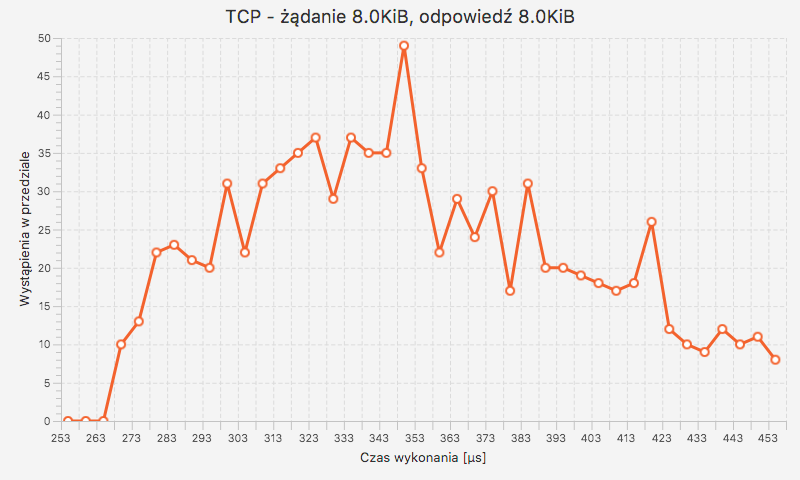
\includegraphics[scale=0.38]{img/charts/TCP_chart_8192_8192.png}
    \caption{Przykładowy wykres rozkładu czasów wykonania dla TCP}
\end{figure}

\begin{figure}[H]
    \centering
    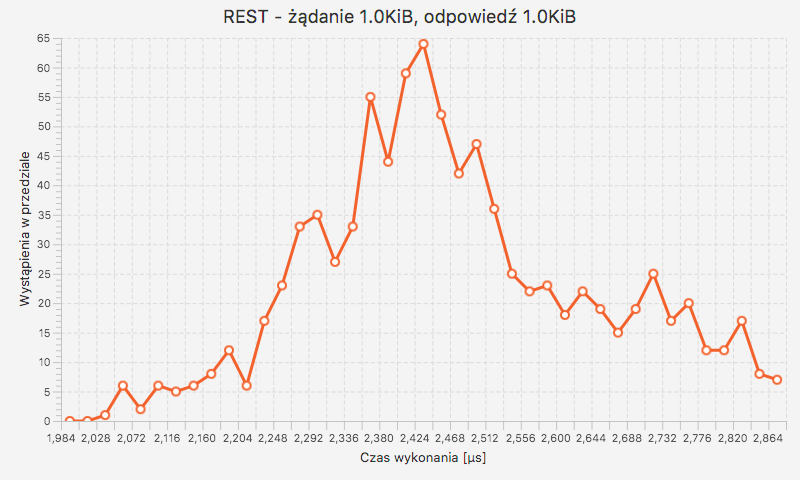
\includegraphics[scale=0.38]{img/charts/REST_chart_1024_1024.png}
    \caption{Przykładowy wykres rozkładu czasów wykonania dla REST}
\end{figure}

\begin{figure}[H]
    \centering
    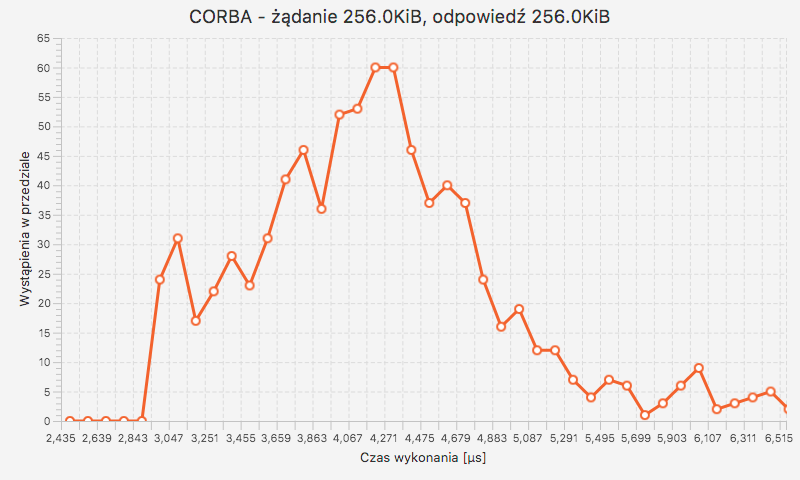
\includegraphics[scale=0.38]{img/charts/CORBA_chart_262144_262144.png}
    \caption{Przykładowy wykres rozkładu czasów wykonania dla technologii CORBA}
\end{figure}

\begin{figure}[H]
    \centering
    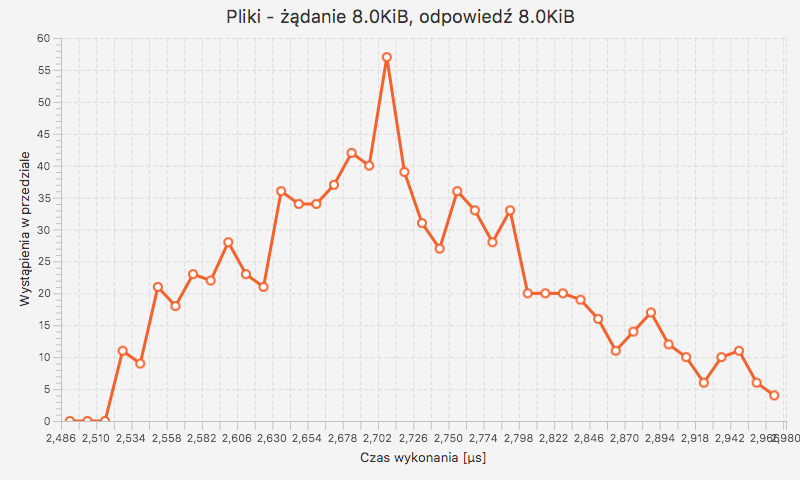
\includegraphics[scale=0.38]{img/charts/FILE_chart_8192_8192.png}
    \caption{Przykładowy wykres rozkładu czasów wykonania dla plików}
\end{figure}

\begin{figure}[H]
    \centering
    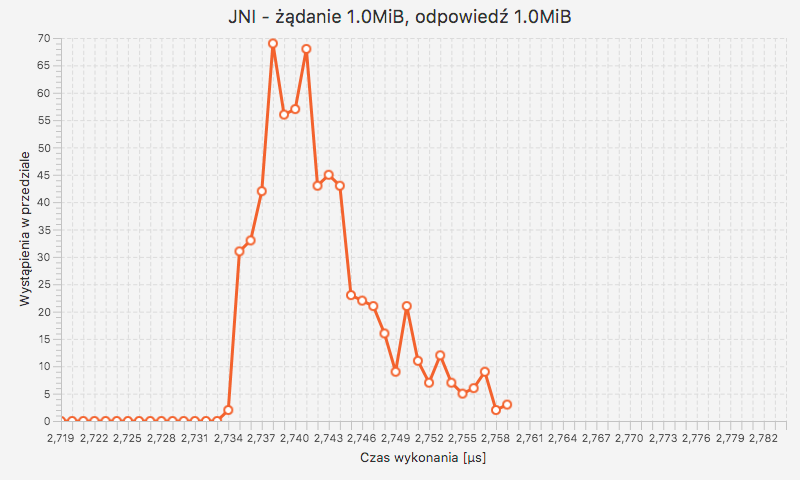
\includegraphics[scale=0.38]{img/charts/JNI_chart_1048576_1048576.png}
    \caption{Przykładowy wykres rozkładu czasów wykonania dla JNI}
\end{figure}


\section{Porównanie wyników}

Najważniejszym zestawieniem jest porównanie czasów komunikacji dla różnych kanałów transmisji danych, przy takim samym rozmiarze przesyłanych danych. Poniżej zaprezentowane zostaną przykładowe wykresy. Z niektórych usunięte zostały najwolniejsze metody, aby dostrzec różnicę między najszybszymi.


\section{tmp}

wnioski z testow:
- wykresy

implementacja - co może jeszcze:
- rozmiar każdej z technologi (np. linie kodu, rozmiar w bajtach)
